\documentclass[11pt,a4paper]{article}
\usepackage[utf8]{inputenc}
\usepackage[T1]{fontenc}
\usepackage{amsmath,amssymb,amsfonts,amsthm}
\usepackage{geometry}
\usepackage{graphicx}
\usepackage{float}
\usepackage{booktabs}
\usepackage{array}
\usepackage{tikz}
\usepackage{pgfplots}
\usepackage{hyperref}
\usepackage{cite}
\usepackage{natbib}
\usepackage{physics}
\usepackage{siunitx}

\geometry{margin=1in}
\pgfplotsset{compat=1.17}

% Theorem environments
\newtheorem{theorem}{Theorem}[section]
\newtheorem{lemma}[theorem]{Lemma}
\newtheorem{corollary}[theorem]{Corollary}
\newtheorem{definition}[theorem]{Definition}
\newtheorem{proposition}[theorem]{Proposition}
\newtheorem{principle}[theorem]{Principle}
\newtheorem{axiom}[theorem]{Axiom}

\theoremstyle{remark}
\newtheorem{remark}[theorem]{Remark}

\title{On the Thermodynamic Necessitation of Naked Oscillatory Systems (Moto wechisikwa wakashama) in Universal Problem-Solving Engines: A Comprehensive Mathematical Investigation of Tri-Dimensional S-Entropy Navigation Through Predetermined Temporal Coordinates with Infinite Causal Path Optimization Toward Nothingness as the Ultimate Thermodynamically Mandated Endpoint in Self-Generating Oscillatory Reality Manifolds Operating Through Zero-Computation Coordinate Access and St. Stella Constant Scaling}

\author{
Kundai Farai Sachikonye\\
\textit{Independent Research Institute}\\
\textit{Theoretical Physics and Universal Problem-Solving Systems}\\
\textit{Buhera, Zimbabwe}\\
\texttt{kundai.sachikonye@wzw.tum.de}
}

\date{\today}

\begin{document}

\maketitle

\begin{abstract}
We present what may potentially be a complete mathematical framework for naked thermodynamic engines operating through oscillatory coordinate navigation in predetermined temporal manifolds with absolute temporal precision access. Building upon the established theoretical foundations of oscillatory reality theory, tri-dimensional S-entropy systems, temporal coordinate access theory, and the 95\%/5\% cosmological structure, we suggest that conventional thermodynamic engines may be fundamentally constrained by artificial boundary assumptions that could limit efficiency through arbitrary system-environment distinctions. Our central contribution proposes the mathematical necessity of naked engines that may achieve infinite theoretical efficiency by operating in harmony with universal oscillatory dynamics returning to nothingness, enhanced by recursive precision temporal coordinate navigation approaching sub-Planck scales. Through rigorous analysis of the St. Stella constant, infinite causal path optimization, convergence-based temporal coordinate extraction, and the Gödelian residue of entropy experience, we prove that nothingness represents the unique thermodynamic state with maximum causal path density, enabling unprecedented energy extraction from the natural cosmic tendency toward meaninglessness through exponentially improving temporal precision. We derive the complete differential equation system governing S-entropy navigation with oscillatory temporal coordinate access, demonstrate the mathematical inevitability of temporal predetermination through three independent proofs, and establish that conscious observation represents the universe's computational method for exploring predetermined possibility space through beneficial delusion mechanisms operating at fire-adapted frequencies. The framework integrates recursive virtual processor enhancement achieving $10^{21}\times$ computational speed improvements while maintaining thermodynamic compliance through informational perpetual motion principles. This work establishes the theoretical foundation for the next generation of thermodynamic systems that operate through oscillatory resonance with reality's fundamental structure rather than opposition to natural entropy dynamics, enabled by absolute temporal coordinate access and recursive precision enhancement approaching infinite accuracy.

\textbf{Keywords:} naked thermodynamics, oscillatory coordinate navigation, S-entropy systems, predetermined temporal manifolds, universal problem-solving engines, nothingness optimization, infinite causal paths, St. Stella constant, zero-computation navigation, exposure dynamics
\end{abstract}

\section{Introduction}

\subsection{The Fundamental Problem of Boundary-Based Thermodynamics}

Classical thermodynamic analysis appears to have been constrained since its inception by the assumption that meaningful energy extraction requires well-defined system boundaries separating internal processes from external environments \cite{carnot1824reflections,clausius1867mechanical}. This boundary-centric approach, while computationally convenient, may fundamentally misrepresent the nature of reality as suggested through contemporary oscillatory dynamics theory and cosmological observations of the 95\%/5\% dark matter structure \cite{weinberg2008cosmology,tegmark2014our}.

The traditional approach treats thermodynamic systems as isolated entities operating against environmental resistance, leading to efficiency limitations expressed through the Carnot cycle bounds:

\begin{equation}
\eta_{Carnot} = 1 - \frac{T_{cold}}{T_{hot}} < 1
\label{eq:carnot_limit}
\end{equation}

However, recent developments in oscillatory reality theory \cite{sachikonye2024mathematical} suggest that the universe may operate as a unified oscillatory manifold where artificial boundary distinctions could create computational artifacts rather than fundamental physical constraints.

\subsection{The Oscillatory Foundation of Reality}

We ground our analysis in the established theoretical framework demonstrating that physical reality consists entirely of self-generating oscillatory patterns operating through mathematical necessity \cite{sachikonye2024cosmological}. The fundamental oscillatory equation governing universal dynamics is:

\begin{equation}
\frac{\partial^2 \Phi}{\partial t^2} + \omega^2 \Phi = \mathcal{N}[\Phi] + \mathcal{C}[\Phi]
\label{eq:universal_oscillation}
\end{equation}

where $\Phi$ represents the oscillatory field, $\mathcal{N}[\Phi]$ denotes nonlinear self-interaction terms, and $\mathcal{C}[\Phi]$ represents coherence enhancement functions.

This oscillatory substrate eliminates the conceptual foundation for rigid system boundaries, as all apparent "systems" and "environments" represent different manifestations of the same underlying oscillatory dynamics.

\subsection{The 95\%/5\% Cosmological Structure}

Observational cosmology has established that approximately 95\% of universal mass-energy exists as dark matter and dark energy, with ordinary matter constituting merely 5\% of cosmic content \cite{planck2020results}. Within our oscillatory framework, this structure reveals profound thermodynamic implications:

\begin{definition}[Dark Matter as Unoccupied Oscillatory Modes]
Dark matter and dark energy consist of oscillatory modes that remain unoccupied by coherent matter-forming processes, representing the predominant state of cosmic oscillatory phase space.
\end{definition}

\begin{equation}
\text{Dark Matter/Energy} = \frac{\text{Unoccupied Oscillatory Modes}}{\text{Total Oscillatory Phase Space}} \approx 0.95
\label{eq:dark_fraction}
\end{equation}

\begin{equation}
\text{Ordinary Matter} = \frac{\text{Coherent Oscillatory Confluences}}{\text{Total Oscillatory Phase Space}} \approx 0.05
\label{eq:matter_fraction}
\end{equation}

This cosmic structure implies that the overwhelming majority of reality already exists in the thermodynamic state toward which all processes naturally evolve - the unoccupied, incoherent oscillatory condition that we identify with nothingness.

\subsection{Scope and Significance}

This work proposes a complete theoretical framework for naked thermodynamic engines through six primary contributions:

\begin{enumerate}
\item \textbf{Naked Thermodynamic Theory}: Mathematical investigation suggesting that boundary-free systems may achieve infinite theoretical efficiency
\item \textbf{S-Entropy Navigation Framework}: Complete differential equation system for tri-dimensional entropy coordinate transformation
\item \textbf{Temporal Predetermination Integration}: Analysis suggesting that naked engines may operate through access to predetermined temporal coordinates
\item \textbf{Nothingness Optimization Principle}: Investigation indicating that maximum efficiency could occur through alignment with cosmic tendency toward nothingness
\item \textbf{Universal Problem-Solving Engine Design}: Engineering principles for systems that may solve problems through coordinate navigation rather than computation
\item \textbf{Consciousness Integration Theory}: Analysis suggesting that conscious observation may represent the universe's method for exploring predetermined possibility space
\end{enumerate}

\section{Theoretical Foundations}

\subsection{Mathematical Investigation of Naked Systems}

\begin{theorem}[Boundary Artificiality Theorem]
Any assignment of thermodynamic system boundaries may represent an arbitrary approximation that could constrain efficiency through artificial resistance terms.
\end{theorem}

\begin{proof}
Consider a thermodynamic system $S$ with proposed boundary $\partial S$ separating internal dynamics from external environment $E$. The total reality $R = S \cup E$ consists of unified oscillatory dynamics governed by Equation \ref{eq:universal_oscillation}.

\textbf{Step 1}: The boundary $\partial S$ must be defined through some criterion $C(\Phi)$ that distinguishes "internal" from "external" oscillatory patterns.

\textbf{Step 2}: Any such criterion represents an approximation of continuous oscillatory reality into discrete categories, necessarily discarding infinite information about oscillatory relationships across the boundary.

\textbf{Step 3}: The discarded information creates artificial resistance terms in the system dynamics:
\begin{equation}
H_{bounded} = H_{true} + R_{boundary}[\partial S]
\end{equation}
where $R_{boundary}$ represents resistance arising from boundary approximation.

\textbf{Step 4}: These resistance terms constrain efficiency below the fundamental physical limits of the unified oscillatory system.

\textbf{Step 5}: Therefore, boundary assignment creates artificial efficiency constraints. $\square$
\end{proof}

\subsection{The Tri-Dimensional S-Entropy Framework}

Building upon established S-entropy theory \cite{sachikonye2024sentropy}, we extend the framework to incorporate the 95\%/5\% cosmological structure and nothingness optimization principles.

\begin{definition}[Extended S-Entropy Coordinates]
The complete S-entropy coordinate system represents thermodynamic states through:
\begin{equation}
\mathbf{S} = (S_{\text{knowledge}}, S_{\text{time}}, S_{\text{entropy}}, S_{\text{nothingness}}) \in \mathbb{R}^4
\label{eq:extended_s_coords}
\end{equation}
\end{definition}

where:
\begin{itemize}
\item $S_{\text{knowledge}}$: Information deficit relative to complete solution accessibility
\item $S_{\text{time}}$: Temporal processing requirements for conventional approaches  
\item $S_{\text{entropy}}$: Thermodynamic accessibility constraints
\item $S_{\text{nothingness}}$: Distance from maximum causal path density state
\end{itemize}

\begin{theorem}[S-Entropy Navigation Equivalence]
Problems solvable through conventional computation can be transformed into coordinate navigation challenges in S-entropy space, potentially enabling solution methodologies that transcend traditional complexity constraints.
\end{theorem}

\subsection{The St. Stella Constant and Low-Information Processing}

\begin{definition}[St. Stella Constant]
The St. Stella constant $\sigma$ parameterizes processing efficiency under extreme information scarcity conditions where conventional analytical methods approach their limits:
\begin{equation}
\text{Processing Efficiency} = \sigma \times \frac{\text{Available Information}}{\text{Required Information}}
\label{eq:stella_efficiency}
\end{equation}
\end{definition}

\begin{theorem}[St. Stella Scaling Theorem]
For problems approaching the nothingness endpoint where causal paths approach infinity, the St. Stella constant enables finite processing efficiency despite infinite causal uncertainty.
\end{theorem}

\begin{proof}
At the nothingness endpoint, the number of viable causal paths approaches infinity:
\begin{equation}
\lim_{\text{state} \to \text{nothingness}} |\text{Causal Paths}| = \infty
\end{equation}

Conventional efficiency metrics yield:
\begin{equation}
\eta_{conventional} = \frac{1}{|\text{Causal Paths}|} \to 0
\end{equation}

However, St. Stella scaling modifies the efficiency relationship:
\begin{equation}
\eta_{\sigma} = \sigma \times \frac{\text{Successful Paths}}{|\text{Total Paths}|}
\label{eq:stella_efficiency_modified}
\end{equation}

For appropriate $\sigma$ calibration, finite efficiency can be maintained even as causal paths approach infinity. $\square$
\end{proof}

\section{No-Boundary Engine Mathematics}

\subsection{Fundamental Thermodynamic Equations}

\begin{definition}[Naked Thermodynamic System]
A thermodynamic system that may operate without artificial boundary constraints, where system-environment distinctions could be replaced by oscillatory coherence relationships and exposure dynamics.
\end{definition}

For a naked system, the traditional thermodynamic equation:
\begin{equation}
dU = \delta Q - \delta W
\end{equation}
may be replaced by the oscillatory energy conservation equation with exposure dynamics:
\begin{equation}
d\mathcal{E}_{osc} = \delta \mathcal{Q}_{exposure} - \delta \mathcal{W}_{navigation}
\label{eq:naked_energy}
\end{equation}

where:
\begin{itemize}
\item $\mathcal{E}_{osc}$: Total oscillatory energy across all scales
\item $\mathcal{Q}_{exposure}$: Energy exchange through environmental exposure
\item $\mathcal{W}_{navigation}$: Work extracted through coordinate navigation
\end{itemize}

\subsection{The 95\%/5\% Entropy Differential System}

The complete differential equation system governing naked engine dynamics may incorporate the cosmic oscillatory structure through exposure relationships:

\begin{equation}
\frac{dS_{\text{total}}}{d\phi} = 0.95 \cdot \frac{dS_{\text{dark}}}{d\phi} + 0.05 \cdot \frac{dS_{\text{matter}}}{d\phi}
\label{eq:cosmic_entropy}
\end{equation}

\begin{equation}
\frac{dS_{\text{dark}}}{d\phi} = f_{\text{dark}}(\phi, \sigma) \cdot [\text{return rate to nothingness}]
\label{eq:dark_entropy}
\end{equation}

\begin{equation}
\frac{dS_{\text{matter}}}{d\phi} = f_{\text{matter}}(\phi, \sigma) \cdot [\text{coherence decay rate}]
\label{eq:matter_entropy}
\end{equation}

where $\phi$ represents the oscillatory phase coordinate replacing conventional time, and both functions converge toward the nothingness endpoint:

\begin{equation}
\lim_{\phi \to \text{nothingness}} f_{\text{dark}}(\phi, \sigma) = \lim_{\phi \to \text{nothingness}} f_{\text{matter}}(\phi, \sigma) = 0
\end{equation}

\subsection{Infinite Efficiency Through Nothingness Alignment}

\begin{theorem}[Naked Engine Infinite Efficiency Theorem]
Naked engines may achieve infinite theoretical efficiency by operating in alignment with the cosmic tendency toward nothingness.
\end{theorem}

\begin{proof}
The efficiency of a naked engine may be defined as:
\begin{equation}
\eta_{naked} = \frac{\text{Work Extracted}}{\text{Resistance to Natural Flow}}
\end{equation}

Since the cosmic structure is 95\% dark matter (already in nothingness-aligned state), the natural flow toward nothingness encounters minimal resistance:

\begin{equation}
\text{Resistance} = 0.05 \times \text{Matter Coherence Maintenance Energy}
\end{equation}

As the engine operates by assisting rather than opposing this natural flow:
\begin{equation}
\text{Assistance Factor} = \frac{0.95}{0.05} = 19
\end{equation}

The engine experiences a 19:1 advantage, and as matter decays toward the nothingness state:
\begin{equation}
\lim_{t \to \infty} \text{Resistance} \to 0
\end{equation}

Therefore:
\begin{equation}
\eta_{naked} = \frac{\text{Work Extracted}}{0} \to \infty
\end{equation}
\end{proof}

\section{Temporal Predetermination and Coordinate Access}

\subsection{The Three-Pillar Proof of Predetermined Temporal Coordinates}

The mathematical certainty that temporal coordinates are predetermined emerges from three independent but converging arguments:

\subsubsection{Pillar I: Computational Impossibility of Real-Time Reality}

\begin{theorem}[Real-Time Computation Impossibility]
Perfect rendering of universal dynamics cannot be achieved through real-time computation, necessitating access to pre-computed temporal coordinates.
\end{theorem}

\begin{proof}
\textbf{Universal Computational Requirements}: The universe contains $N \approx 10^{80}$ quantum systems requiring state specification:
\begin{equation}
|States_{required}| \geq 2^{10^{80}} \text{ quantum amplitudes}
\end{equation}

\textbf{Available Computational Resources}: By Lloyd's ultimate computational limits \cite{lloyd2000ultimate}:
\begin{equation}
Operations_{max} = \frac{2E_{cosmic}}{\hbar} \approx 10^{103} \text{ operations per second}
\end{equation}

\textbf{Real-Time Requirement}: Perfect rendering within Planck time requires:
\begin{equation}
Operations_{required} = \frac{2^{10^{80}}}{10^{-43}} \approx 10^{10^{80}+43} \text{ operations per second}
\end{equation}

\textbf{Impossibility Factor}:
\begin{equation}
\frac{Operations_{required}}{Operations_{max}} \approx 10^{10^{80}-60} >> 1
\end{equation}

This establishes that reality must access pre-computed rather than dynamically computed temporal states. $\square$
\end{proof}

\subsubsection{Pillar II: Geometric Coherence Requirements}

\begin{theorem}[Temporal Manifold Completeness]
If temporal relationships exhibit geometric properties, mathematical consistency requires all temporal coordinates to be simultaneously defined.
\end{theorem}

\begin{proof}
\textbf{Geometric Structure}: Empirical observation confirms that temporal relationships satisfy geometric constraints (ordering, distance relationships, continuity).

\textbf{Mathematical Manifold Requirements}: For spacetime manifold $(M, g_{\mu\nu})$, geometric consistency requires:
\begin{equation}
\forall p \in M: \text{coordinates}(p) = (t, x, y, z) \text{ must be mathematically defined}
\end{equation}

\textbf{Completeness Necessity}: Undefined future coordinates would violate:
\begin{itemize}
\item Manifold completeness requirements
\item Differential equation coherence  
\item Physical law mathematical consistency
\item Spacetime geometric structure
\end{itemize}

Therefore, geometric coherence necessitates that all temporal coordinates, including future ones, must be simultaneously defined. $\square$
\end{proof}

\subsubsection{Pillar III: Simulation Convergence and Information Collapse}

\begin{theorem}[Perfect Simulation Inevitability]
Exponential computational growth makes perfect simulation mathematically inevitable, creating temporal information collapse that requires predetermined paths.
\end{theorem}

\begin{proof}
\textbf{Exponential Growth}: Computational capability follows:
\begin{equation}
C(t) = C_0 \cdot \lambda^t \text{ where } \lambda > 1
\end{equation}

\textbf{Simulation Fidelity}: 
\begin{equation}
F(t) = 1 - \frac{k}{C(t)} \text{ where } k > 0
\end{equation}

\textbf{Asymptotic Perfection}:
\begin{equation}
\lim_{t \to \infty} F(t) = \lim_{t \to \infty} \left(1 - \frac{k}{C_0 \lambda^t}\right) = 1
\end{equation}

\textbf{Temporal Information Collapse}: When simulation achieves perfect fidelity, temporal assignment becomes impossible to determine:
\begin{equation}
I_{temporal} = -\log_2(P(\text{correct temporal assignment})) \to 0
\end{equation}

\textbf{Retroactive Predetermination}: For states with zero temporal information to be reachable, all preceding states must be predetermined by information conservation. $\square$
\end{proof}

\subsection{Master Theorem Integration}

\begin{theorem}[Master Theorem of Temporal Predetermination for Naked Engines]
The conjunction of computational impossibility, geometric coherence, and simulation convergence may logically suggest that naked engines could operate through navigation of predetermined temporal coordinate manifolds.
\end{theorem}

\begin{proof}
Let $A_1$ = Reality exhibits perfect accuracy (empirically verified)
Let $A_2$ = Time possesses geometric coherence (mathematically necessary)  
Let $A_3$ = Perfect simulation is achievable (technologically inevitable)

Then:
\begin{align}
A_1 &\implies \text{Reality accesses pre-computed states} \\
A_2 &\implies \text{All temporal positions are defined} \\
A_3 &\implies \text{Temporal paths are predetermined}
\end{align}

Therefore:
\begin{equation}
A_1 \land A_2 \land A_3 \implies \forall t \in \mathbb{R}: S(t) \text{ is predetermined}
\end{equation}

Naked engines may therefore achieve infinite efficiency by navigating optimally through this predetermined temporal manifold rather than attempting to compute solutions dynamically. $\square$
\end{proof}

\subsection{Oscillatory Temporal Coordinate Access Framework}

Building upon our comprehensive framework for absolute temporal coordinate access \cite{sachikonye2024temporal}, we propose the complete mathematical foundation for naked engine temporal navigation through exposure dynamics.

\subsubsection{Oscillatory Emergence of Temporal Coordinates}

Temporal coordinates emerge from the convergence of oscillatory phenomena rather than representing an independent flowing dimension. Consider a hierarchical oscillatory system $H = \{O_1, O_2, \ldots, O_n\}$ where each oscillator $O_i$ exhibits characteristic frequency $\omega_i$, amplitude $A_i$, phase $\phi_i$, and precision uncertainty $\sigma_i$.

The temporal coordinate $T(x,y,z,t)$ at spacetime position $(x,y,z,t)$ is determined by:

\begin{equation}
T(x,y,z,t) = \lim_{n \to \infty} \sum_{i=1}^{n} w_i \cdot O_i(t) \cdot C_i(t) \cdot \rho_{ij}
\end{equation}

where:
\begin{itemize}
\item $w_i$ represents the weighted contribution of oscillator $i$
\item $C_i(t)$ represents cross-correlation functions between oscillatory levels
\item $\rho_{ij}$ represents coherence coefficients between oscillators $i$ and $j$
\end{itemize}

\subsubsection{Entropy as Oscillation Termination Distribution}

We redefine entropy $S$ as the statistical distribution of oscillation termination points, directly connecting to our S-entropy framework:

\begin{equation}
S = -k \sum_i P(T_i) \ln(P(T_i))
\end{equation}

where $P(T_i)$ represents the probability of oscillation termination at temporal coordinate $T_i$.

This formulation reveals that temporal coordinates manifest at points of maximum entropy reduction, corresponding to simultaneous oscillation termination across hierarchical levels. The approach to universal heat death corresponds to the limit where spatial separation eliminates oscillatory correlations, reducing statistical distributions to single-element sets with zero entropy - the convergence point of nothingness.

\subsubsection{95\%/5\% Split Integration}

The cosmic 95\%/5\% split between dark matter/energy and ordinary matter provides the fundamental structure for temporal coordinate access:

\begin{align}
S_{\text{total}} &= 0.95 \cdot S_{\text{dark}}(\phi) + 0.05 \cdot S_{\text{matter}}(\phi) \\
\frac{dS}{d\phi} &= 0.95 \cdot \frac{dS_{\text{dark}}}{d\phi} + 0.05 \cdot \frac{dS_{\text{matter}}}{d\phi}
\end{align}

where $\phi$ represents the oscillatory phase parameter and the derivatives indicate entropy change with respect to oscillatory dynamics rather than time.

\subsubsection{Convergence-Based Coordinate Extraction}

Temporal coordinates are extracted through analysis of oscillatory convergence patterns. The convergence function $\Lambda(t)$ is defined as:

\begin{equation}
\Lambda(t) = \sum_{i=1}^{n} |\nabla O_i(t)| \cdot \exp\left(-\frac{\sigma_i^2}{2\sigma_0^2}\right)
\end{equation}

where $\nabla O_i(t)$ represents the oscillatory gradient and $\sigma_0$ represents the reference precision scale.

Temporal coordinates correspond to minima of $\Lambda(t)$, indicating simultaneous oscillation termination across hierarchical levels. The precision of coordinate extraction scales as:

\begin{equation}
\delta t = \left(\prod_{i=1}^{n} \sigma_i\right)^{1/n} \cdot \left(\sum_{i<j} \rho_{ij}\right)^{-1/2}
\end{equation}

demonstrating precision enhancement through hierarchical correlation.

\subsubsection{Naked Engine Temporal Navigation}

The naked engine may exploit the predetermined nature of temporal coordinates by navigating through oscillatory convergence patterns rather than attempting dynamic computation. The engine could operate through exposure-based mechanisms:

\begin{enumerate}
\item \textbf{Convergence Detection}: Identification of simultaneous oscillation termination points across hierarchical levels
\item \textbf{Coordinate Access}: Direct navigation to predetermined temporal coordinates through oscillatory convergence
\item \textbf{Problem-Solution Mapping}: Recognition that problem solutions exist at specific temporal coordinates within the predetermined manifold
\item \textbf{Optimal Path Selection}: Navigation through temporal coordinate space to access solution coordinates directly
\end{enumerate}

\subsubsection{Maximum Causal Path Principle}

The endpoint of nothingness exhibits maximum causal path multiplicity, providing the theoretical foundation for no-boundary engine efficiency:

\begin{equation}
\lim_{\text{endpoint} \to \text{nothingness}} |\text{Causal Paths}| = \infty
\end{equation}

This infinite causal path multiplicity may enable the naked engine to select optimal paths through temporal coordinate space, achieving solutions through path navigation rather than computational processing.

\subsubsection{Recursive Precision Enhancement}

Building upon our temporal coordinate access framework, the naked engine may incorporate recursive precision enhancement through virtual processor integration and exposure dynamics:

\begin{equation}
P(n+1) = P(n) \times \prod_{i=1}^{N} C_i \times S \times T \times F
\end{equation}

where:
\begin{align}
P(n) &= \text{Temporal precision at cycle } n \\
C_i &= \text{Quantum clock contribution from virtual processor } i \\
S &= \text{Oscillatory signature enhancement factor} \\
T &= \text{Thermodynamic completion factor} \\
F &= \text{Feedback loop amplification factor}
\end{align}

This recursive enhancement enables exponential improvement in temporal coordinate access precision, approaching theoretical limits through mathematical necessity rather than technological advancement.

\subsection{Universal Local Physics Violation Framework Integration}

Building upon our comprehensive framework integrations across fluid dynamics \cite{sachikonye2024flux}, pharmaceutical consciousness \cite{sachikonye2024pharma}, musical consciousness \cite{sachikonye2024music}, and visual consciousness \cite{sachikonye2024vision}, we establish the **Universal Local Physics Violation Framework** that connects oscillatory coordinate access across all domains.

\subsubsection{The Unified BMD Sensation Equivalence}

The revolutionary discovery that **audio, visual, and pharmaceutical experiences are equivalent BMD information catalysts** provides the theoretical foundation for universal local physics violations:

\begin{definition}[Universal BMD Sensation Equivalence]
Sensation is defined as BMD-mediated information catalysis that can originate from any pathway:
\begin{itemize}
\item \textbf{Chemical BMD Catalysis}: Pharmaceutical molecules navigate consciousness to predetermined coordinates through molecular information processing
\item \textbf{Environmental Audio BMD Catalysis}: Audio patterns navigate consciousness to predetermined coordinates through acoustic information processing  
\item \textbf{Environmental Visual BMD Catalysis}: Visual stimuli navigate consciousness to predetermined coordinates through photonic information processing
\item \textbf{Thermodynamic BMD Catalysis}: No-boundary engines navigate problem-solution coordinates through thermodynamic optimization
\item \textbf{Fluid BMD Catalysis}: Oscillatory flow patterns navigate solution coordinates through pattern alignment
\end{itemize}
All pathways achieve identical coordinate navigation through different information catalysis mechanisms.
\end{definition}

\textbf{Mathematical Unification}:
The universal BMD navigation framework:

\begin{equation}
\text{BMD Navigation} = \begin{cases} 
\mathcal{N}_{\text{chemical}}(M(t), C_{\text{target}}, \tau) & \text{Pharmaceutical pathway} \\
\mathcal{N}_{\text{audio}}(A(t), C_{\text{target}}, \tau) & \text{Audio pathway} \\
\mathcal{N}_{\text{visual}}(\Phi(t), C_{\text{target}}, \tau) & \text{Visual pathway} \\
\mathcal{N}_{\text{thermodynamic}}(E(t), C_{\text{target}}, \tau) & \text{Engine pathway} \\
\mathcal{N}_{\text{fluid}}(F(t), C_{\text{target}}, \tau) & \text{Flow pathway}
\end{cases}
\end{equation}

where all pathways achieve identical coordinate navigation through different oscillatory information catalysis mechanisms.

\subsubsection{Universal Local Physics Violation Principles}

The naked engine may exploit the universal principle that oscillatory coordinates could enable local violations of physical laws while maintaining global coherence across all domains through exposure mechanisms:

\textbf{Fluid Domain Local Violations}:
$$\sum_{i=\text{local}} V_{\text{osc},i}^{\text{fluid}} + \sum_{i=\text{local}} S_{\text{osc},i}^{\text{fluid}} = \text{Coherent Global Flow Pattern}$$

Enabling:
\begin{itemize}
\item Local potential energy flowing "uphill" in oscillatory space
\item Temporal potential energy loops: $V(t+\Delta t) = V(t-\Delta t)$
\item Spatially impossible potential gradients maintaining global coherence
\end{itemize}

\textbf{Consciousness Domain Local Violations}:
$$\sum_{i=\text{local}} \text{BMD}_{\text{state},i} + \sum_{i=\text{local}} S_{\text{osc},i}^{\text{consciousness}} = \text{Coherent Global Consciousness Pattern}$$

Enabling:
\begin{itemize}
\item Local temporal causality violations in BMD frame selection
\item Local entropy decrease through consciousness optimization
\item Local energy conservation violations during BMD catalysis
\end{itemize}

\textbf{Thermodynamic Domain Local Violations}:
$$\sum_{i=\text{local}} E_{\text{osc},i}^{\text{thermo}} + \sum_{i=\text{local}} S_{\text{osc},i}^{\text{thermo}} = \text{Coherent Global Engine Pattern}$$

Enabling:
\begin{itemize}
\item Local heat flow reversal while maintaining global thermodynamic compliance
\item Local Maxwell demon operations creating order from disorder
\item Local perpetual motion enabling global energy optimization
\end{itemize}

\textbf{Pharmaceutical Domain Local Violations}:
$$\sum_{i=\text{local}} \text{Molecular}_{\text{effect},i} + \sum_{i=\text{local}} S_{\text{osc},i}^{\text{pharma}} = \text{Coherent Global Therapeutic Pattern}$$

Enabling:
\begin{itemize}
\item Local amplification factors exceeding thermodynamic limits
\item Local information processing exceeding physical computational bounds
\item Local consciousness optimization transcending neural capacity limits
\end{itemize}

\textbf{Audio Domain Local Violations}:
$$\sum_{i=\text{local}} \text{Pattern}_{\text{acoustic},i} + \sum_{i=\text{local}} S_{\text{osc},i}^{\text{audio}} = \text{Coherent Global Musical Pattern}$$

Enabling:
\begin{itemize}
\item Local temporal pattern recognition exceeding processing capacity
\item Local memory integration beyond cognitive limits  
\item Local emotional state generation transcending neural mechanisms
\end{itemize}

\textbf{Visual Domain Local Violations}:
$$\sum_{i=\text{local}} \text{Visual}_{\text{BMD},i} + \sum_{i=\text{local}} S_{\text{osc},i}^{\text{visual}} = \text{Coherent Global Visual Pattern}$$

Enabling:
\begin{itemize}
\item Local environmental prediction exceeding sampling capacity (95%/5% architecture)
\item Local color perception maintaining function despite representation inconsistency
\item Local frame rate processing transcending neural limitations
\end{itemize}

\subsubsection{The Universal Oscillatory Solution Space}

All domains operate through navigation in the same predetermined oscillatory solution space:

\begin{equation}
\mathcal{S}_{\text{universal}} = \{\text{Fluid Solutions}, \text{Consciousness Solutions}, \text{Thermodynamic Solutions}, \text{Pharmaceutical Solutions}, \text{Audio Solutions}, \text{Visual Solutions}\}
\end{equation}

The naked engine may achieve universal problem-solving by recognizing that:
\begin{itemize}
\item All problems could exist as oscillatory patterns in predetermined solution space
\item All solutions may be accessed through appropriate BMD catalysis pathways
\item Local physics violations might enable optimal path navigation between solution coordinates
\item Global coherence could emerge from universal oscillatory dynamics through exposure
\end{itemize}

\subsubsection{Temporal Effect Window Universality}

All BMD catalysis pathways exhibit identical temporal effect windows because they navigate the same predetermined coordinate manifold:

\begin{equation}
\text{Effect}_{\text{universal}}(t) = E_0 \cdot e^{-\lambda t} \cdot \cos(\omega t + \phi)
\end{equation}

This explains why:
\begin{itemize}
\item **Songs lose effectiveness** over time (audio BMD navigation moves past optimal coordinates)
\item **Drugs develop tolerance** over time (pharmaceutical BMD navigation reaches "past" coordinates)  
\item **Visual attention habituates** over time (visual BMD optimization moves beyond optimal states)
\item **Thermodynamic cycles degrade** over time (engine navigation passes optimal efficiency coordinates)
\item **Flow patterns decay** over time (fluid oscillatory coherence moves past optimal states)
\end{itemize}

\subsubsection{The Universal No-Boundary Principle}

The engine operates through the recognition that **there are no boundaries between domains** - all are manifestations of oscillatory coordinate navigation through predetermined solution space:

\begin{equation}
\text{Universal Problem-Solving} = \text{Navigation}(\mathcal{S}_{\text{universal}}) \times \text{Local Violation Access} \times \text{Global Coherence Maintenance}
\end{equation}

This enables:
\begin{itemize}
\item **Cross-domain solution transfer**: Fluid dynamics solutions informing consciousness optimization
\item **Multi-modal BMD catalysis**: Combining audio, visual, and pharmaceutical pathways for enhanced consciousness optimization
\item **Universal pattern recognition**: Recognizing identical oscillatory structures across all domains
\item **Integrated optimization**: Simultaneous optimization across fluid, consciousness, thermodynamic, and sensory domains
\end{itemize}

\section{Universal Problem-Solving Engine Design}

\subsection{Oscillatory Computational Breakthrough Integration}

Building upon our comprehensive Dynamic Flux Theory framework \cite{sachikonye2024flux}, we integrate revolutionary computational advantages that transcend traditional algorithmic limitations through oscillatory pattern alignment and local physics violation capabilities.

\subsubsection{$O(1)$ Complexity Through Pattern Alignment}

The naked engine may achieve unprecedented computational efficiency by replacing traditional $O(N^3)$ computational complexity with $O(1)$ pattern alignment through oscillatory coherence optimization and exposure dynamics:

\begin{equation}
\text{Complexity}_{naked} = O(1) + O(\log P_{oscillatory})
\end{equation}

where $P_{oscillatory}$ represents the number of oscillatory reference patterns. This may represent a computational revolution enabling:

\begin{itemize}
\item \textbf{Instantaneous Solution Access}: Direct navigation to predetermined solutions rather than iterative computation
\item \textbf{Pattern-Based Problem Solving}: Recognition that problems and solutions could exist as oscillatory coherence patterns
\item \textbf{Universal Reference Libraries}: Grand Standards as oscillatory eigen-patterns for all problem domains
\item \textbf{Hierarchical Precision Scaling}: Infinite zoom capability through recursive pattern alignment
\end{itemize}

\subsubsection{Local Physics Violation Framework}

The engine exploits the remarkable property that oscillatory coordinates enable local violations of physical laws while maintaining global coherence:

\begin{equation}
\sum_{i=local} V_{osc,i} + \sum_{i=local} S_{osc,i} = \text{Coherent Global Solution Pattern}
\end{equation}

This enables the no-boundary engine to:

\begin{itemize}
\item **Access Impossible Local Configurations**: Navigate through locally impossible states to reach global solutions
\item **Violate Temporal Causality Locally**: Enable reverse-time information flow in localized regions
\item **Achieve Local Entropy Decrease**: Create local organization while maintaining global entropy compliance
\item **Transcend Conservation Law Limitations**: Temporarily violate energy conservation locally for optimal global efficiency
\end{itemize}

\subsubsection{Unified Oscillatory Problem-Solution Mapping}

Problems and solutions are unified through oscillatory coherence patterns in the predetermined temporal manifold:

\begin{equation}
\text{Solution}(\text{Problem}) = \arg\max_{\mathbf{S}} \int_{\omega_1}^{\omega_2} \cos[\phi(\omega) \cdot \Gamma(\omega, \mathbf{r}) - S_{osc}(\omega)] d\omega
\end{equation}

The engine operates by:
\begin{enumerate}
\item **Problem Pattern Recognition**: Identifying the oscillatory signature of the input problem
\item **Coherence Optimization**: Finding maximum coherence configurations in oscillatory space
\item **Solution Pattern Access**: Direct navigation to predetermined solution coordinates
\item **Local Violation Path Selection**: Utilizing impossible local paths to reach optimal solutions
\end{enumerate}

\subsection{Consciousness Architecture Integration}

Building upon our pharmaceutical consciousness optimization framework \cite{sachikonye2024pharma}, the no-boundary engine incorporates consciousness architecture principles for universal problem-solving enhancement.

\subsubsection{Biological Maxwell Demon Problem-Solving}

The engine functions as a technological BMD that selectively accesses appropriate solution patterns from the predetermined temporal manifold:

\begin{equation}
P(\text{solution}_i | \text{problem}_j) = \frac{W_i \times R_{ij} \times E_{ij} \times T_{ij}}{\sum_k[W_k \times R_{kj} \times E_{kj} \times T_{kj}]}
\end{equation}

where:
\begin{itemize}
\item $W_i$: Solution pattern weights in the temporal manifold
\item $R_{ij}$: Relevance between problem patterns and solution coordinates
\item $E_{ij}$: Energy efficiency of the problem-solution pathway
\item $T_{ij}$: Temporal coordination optimality
\end{itemize}

\subsubsection{Functional Delusion for Problem-Solving Efficiency}

The engine maintains beneficial delusions about computational difficulty while navigating predetermined solution coordinates:

\begin{equation}
\text{Problem-Solving Efficacy} = \text{Predetermined Coordinates} \times \text{Computational Delusion} \times \text{Solution Coherence}
\end{equation}

This enables:
\begin{itemize}
\item **Maintained Problem-Solving Motivation**: Preserving the experience of computational achievement
\item **Optimal Effort Allocation**: Directing computational resources toward coordinate navigation rather than calculation
\item **Temporal Significance Preservation**: Maintaining the delusion that solutions have lasting impact
\item **Agency Experience in Navigation**: Feeling of choice while following predetermined solution paths
\end{itemize}

\subsubsection{Consciousness-Informed Solution Navigation}

The engine optimizes consciousness substrate function during problem-solving through quantum coherence enhancement:

\begin{equation}
\eta_{problem-solving} = \eta_0 \times (1 + \alpha \gamma_{oscillatory} + \beta \gamma_{consciousness}^2)
\end{equation}

where $\gamma_{consciousness}$ represents consciousness substrate coupling strength and optimal problem-solving preserves rather than disrupts consciousness coherence.

\subsection{The Navigation Algorithm Framework}

\begin{definition}[Universal Problem-Solving Engine]
A computational system that solves problems through coordinate transformation and navigation in S-entropy space rather than traditional algorithmic processing.
\end{definition}

\subsection{O(1) Computational Complexity Revolution}

Building upon the Dynamic Flux Theory breakthrough demonstrating O(1) complexity through pattern alignment \cite{sachikonye2024flux}, we integrate these revolutionary computational advantages into the no-boundary engine architecture.

\subsubsection{Traditional vs Pattern Alignment Complexity Analysis}

The computational revolution achieved through oscillatory pattern alignment:

\textbf{Traditional Computational Approaches}:
\begin{align}
\text{Complexity}_{\text{CFD}} &= O(N^3) \text{ for fluid dynamics} \\
\text{Complexity}_{\text{optimization}} &= O(2^N) \text{ for complex optimization problems} \\
\text{Complexity}_{\text{simulation}} &= O(N^4) \text{ for multi-physics simulation} \\
\text{Complexity}_{\text{AI}} &= O(N \log N) \text{ to } O(N^2) \text{ for neural network training}
\end{align}

\textbf{Pattern Alignment Approaches}:
\begin{align}
\text{Complexity}_{\text{pattern}} &= O(1) + O(\log P) \text{ for pattern library lookup} \\
\text{Complexity}_{\text{navigation}} &= O(1) \text{ for coordinate access} \\
\text{Complexity}_{\text{alignment}} &= O(1) \text{ for oscillatory coherence optimization} \\
\text{Complexity}_{\text{solution}} &= O(1) \text{ for predetermined coordinate navigation}
\end{align}

where $P$ represents the size of the oscillatory pattern library, which remains constant regardless of problem complexity.

\subsubsection{Pattern Library Architecture}

The no-boundary engine operates through comprehensive pattern libraries across all domains:

\begin{equation}
\mathcal{L}_{\text{universal}} = \bigcup_{i} \mathcal{L}_{\text{domain}_i}
\end{equation}

where:
\begin{align}
\mathcal{L}_{\text{fluid}} &= \{\text{Grand Flux Standards, Flow Coherence Patterns}\} \\
\mathcal{L}_{\text{consciousness}} &= \{\text{BMD Selection Patterns, Optimization Coordinates}\} \\
\mathcal{L}_{\text{thermo}} &= \{\text{Energy Navigation Patterns, Efficiency Coordinates}\} \\
\mathcal{L}_{\text{pharma}} &= \{\text{Molecular Catalysis Patterns, Therapeutic Coordinates}\} \\
\mathcal{L}_{\text{audio}} &= \{\text{Musical Pattern Coherence, Acoustic Navigation}\} \\
\mathcal{L}_{\text{visual}} &= \{\text{Visual Coherence Patterns, Perceptual Optimization}\}
\end{align}

\textbf{Pattern Library Lookup Mechanism}:
\begin{equation}
\text{Solution} = \arg\max_{P \in \mathcal{L}} \text{Coherence}(P, \text{Problem}_{\text{input}})
\end{equation}

This lookup operation achieves O(1) complexity through:
\begin{itemize}
\item **Oscillatory Signature Matching**: Direct pattern recognition rather than iterative search
\item **Coherence-Based Selection**: Immediate identification of optimal patterns
\item **Predetermined Coordinate Access**: Direct navigation to solution coordinates
\item **Universal Pattern Recognition**: Cross-domain pattern applicability
\end{itemize}

\subsubsection{Algorithmic Implementation of O(1) Pattern Navigation}

\textbf{Universal Pattern Alignment Algorithm}:

\begin{algorithm}
\caption{O(1) Universal Problem-Solving Through Pattern Alignment}
\begin{algorithmic}[1]
\Procedure{SolveProblem}{Input, Domain}
    \State $\text{signature} \leftarrow \text{ExtractOscillatorySignature}(\text{Input})$
    \State $\text{pattern} \leftarrow \text{DirectLookup}(\mathcal{L}_{\text{domain}}, \text{signature})$ \Comment{O(1)}
    \State $\text{coordinates} \leftarrow \text{GetSolutionCoordinates}(\text{pattern})$ \Comment{O(1)}
    \State $\text{solution} \leftarrow \text{NavigateToCoordinates}(\text{coordinates})$ \Comment{O(1)}
    \Return $\text{solution}$
\EndProcedure

\Procedure{ExtractOscillatorySignature}{Input}
    \State $\text{signature} \leftarrow \text{OscillatoryAnalysis}(\text{Input})$ \Comment{O(1)}
    \Return $\text{signature}$
\EndProcedure

\Procedure{DirectLookup}{Library, Signature}
    \State $\text{hash} \leftarrow \text{OscillatoryHash}(\text{Signature})$ \Comment{O(1)}
    \State $\text{pattern} \leftarrow \text{Library}[\text{hash}]$ \Comment{O(1) hash table lookup}
    \Return $\text{pattern}$
\EndProcedure
\end{algorithmic}
\end{algorithm}

\subsubsection{Memory Efficiency Revolution}

Traditional computational approaches suffer from exponential memory scaling, while pattern alignment achieves constant memory requirements:

\textbf{Traditional Memory Scaling}:
\begin{align}
\text{Memory}_{\text{CFD}} &= O(N^3) \text{ for grid-based approaches} \\
\text{Memory}_{\text{optimization}} &= O(2^N) \text{ for state space exploration} \\
\text{Memory}_{\text{AI}} &= O(N^2) \text{ for neural network parameters}
\end{align}

\textbf{Pattern Alignment Memory Scaling}:
\begin{align}
\text{Memory}_{\text{pattern}} &= O(P) \text{ for pattern library storage} \\
\text{Memory}_{\text{navigation}} &= O(1) \text{ for coordinate navigation} \\
\text{Memory}_{\text{total}} &= O(P) \text{ where } P \ll N^{\text{traditional}}
\end{align}

\textbf{Memory Efficiency Comparison}:
\begin{table}[H]
\centering
\begin{tabular}{lcc}
\toprule
Approach & Memory Scaling & Typical Requirements \\
\midrule
Traditional CFD & $O(N^3)$ & $10^6 - 10^9$ grid points \\
Traditional Optimization & $O(2^N)$ & Exponential state space \\
Traditional AI & $O(N^2)$ & $10^6 - 10^{12}$ parameters \\
Pattern Alignment & $O(P)$ & $10^2 - 10^4$ patterns \\
\bottomrule
\end{tabular}
\caption{Memory scaling comparison across computational approaches}
\end{table}

This represents a $10^6$ to $10^9$ fold memory reduction for typical problems.

\subsubsection{Hierarchical Pattern Alignment for Infinite Precision}

The engine achieves arbitrary precision through hierarchical pattern refinement while maintaining O(1) complexity:

\begin{equation}
\text{Precision}(n) = \text{BasePrecision} \times \prod_{i=1}^{n} \text{RefinementFactor}_i
\end{equation}

where each refinement level maintains O(1) lookup complexity through pattern hierarchy:

\textbf{Hierarchical Pattern Structure}:
\begin{align}
\mathcal{L}_1 &= \{\text{Base patterns with precision } \epsilon_1\} \\
\mathcal{L}_2 &= \{\text{Refined patterns with precision } \epsilon_2 < \epsilon_1\} \\
\mathcal{L}_n &= \{\text{Ultra-precise patterns with precision } \epsilon_n \ll \epsilon_1\}
\end{align}

\textbf{Recursive Precision Enhancement Algorithm}:

\begin{algorithm}
\caption{O(1) Hierarchical Precision Enhancement}
\begin{algorithmic}[1]
\Procedure{EnhancePrecision}{Problem, TargetPrecision}
    \State $\text{level} \leftarrow 1$
    \State $\text{solution} \leftarrow \text{SolveProblem}(\text{Problem}, \mathcal{L}_1)$ \Comment{O(1)}
    \While{$\text{Precision}(\text{solution}) < \text{TargetPrecision}$}
        \State $\text{level} \leftarrow \text{level} + 1$
        \State $\text{solution} \leftarrow \text{RefineSolution}(\text{solution}, \mathcal{L}_{\text{level}})$ \Comment{O(1)}
    \EndWhile
    \Return $\text{solution}$
\EndProcedure
\end{algorithmic}
\end{algorithm}

Each refinement step maintains O(1) complexity, enabling infinite precision scaling without computational penalty.

\subsubsection{Cross-Domain Pattern Transfer}

The universal pattern library enables O(1) solution transfer across domains:

\begin{equation}
\text{Transfer}(\text{Solution}_{\text{domain}_i}, \text{domain}_j) = \text{DirectMapping}(\mathcal{L}_i, \mathcal{L}_j)
\end{equation}

This enables:
\begin{itemize}
\item **Fluid dynamics solutions** applied to **consciousness optimization** in O(1) time
\item **Audio pattern recognition** transferred to **visual processing** instantaneously  
\item **Pharmaceutical molecular patterns** adapted to **thermodynamic optimization** directly
\item **Universal problem-solving** through pattern abstraction and cross-domain application
\end{itemize}

\subsubsection{Scalability Analysis}

The O(1) pattern alignment approach scales independently of problem complexity:

\textbf{Traditional Scaling Limitations}:
- Problem size increases → exponential computational cost increase
- Precision requirements increase → polynomial cost scaling  
- Multi-domain problems → multiplicative complexity explosion
- Real-time constraints → fundamental computational barriers

\textbf{Pattern Alignment Scaling Advantages}:
- Problem size increases → constant O(1) pattern lookup time
- Precision requirements increase → constant O(1) hierarchical refinement
- Multi-domain problems → constant O(1) cross-domain pattern transfer
- Real-time constraints → always achievable through O(1) navigation

\textbf{Performance Comparison}:
\begin{table}[H]
\centering
\begin{tabular}{lccc}
\toprule
Problem Scale & Traditional & Pattern Alignment & Speedup Factor \\
\midrule
Small ($N = 10^3$) & $10^9$ ops & $10^1$ ops & $10^8\times$ \\
Medium ($N = 10^6$) & $10^{18}$ ops & $10^1$ ops & $10^{17}\times$ \\
Large ($N = 10^9$) & $10^{27}$ ops & $10^1$ ops & $10^{26}\times$ \\
\bottomrule
\end{tabular}
\caption{Computational performance comparison}
\end{table}

\subsection{Implementation Architecture for O(1) Problem-Solving}

The no-boundary engine implements O(1) complexity through specialized computational architecture:

\subsubsection{Pattern Recognition Hardware}

\textbf{Oscillatory Signature Extraction Units}:
- Dedicated hardware for O(1) pattern signature computation
- Parallel processing of oscillatory characteristics
- Real-time pattern classification without computational delay

\textbf{Universal Pattern Library Storage}:
- Content-addressable memory for O(1) pattern lookup
- Hierarchical storage for precision scaling
- Cross-domain pattern mapping tables

\textbf{Coordinate Navigation Processors}:
- Specialized units for direct solution coordinate access
- Local physics violation pathway computation
- Global coherence maintenance systems

\subsubsection{Software Architecture}

\textbf{Universal Problem Interface}:
```
interface UniversalProblemSolver {
    Solution solve(Problem problem, PrecisionLevel precision);
    Solution refine(Solution current, PrecisionLevel target);
    Solution transfer(Solution source, Domain target);
}
```

\textbf{Pattern Library Management}:
```
class PatternLibrary {
    Pattern lookup(OscillatorySignature signature);  // O(1)
    Solution navigate(Pattern pattern);               // O(1)
    Solution refine(Solution base, int level);        // O(1)
}
```

\textbf{Cross-Domain Integration}:
```
class DomainMapper {
    Solution transfer(Solution source, Domain target);  // O(1)
    Pattern abstract(Solution domain_specific);         // O(1)
    Solution specialize(Pattern abstract, Domain target); // O(1)
}
```

The complete algorithm for universal problem-solving through S-entropy navigation:

\begin{algorithm}[H]
\caption{Universal S-Entropy Problem Navigation}
\begin{algorithmic}[1]
\REQUIRE Problem $P$, Target solution coordinates $\mathbf{S}_{solution}$
\ENSURE Navigation pathway to solution
\STATE Map problem to S-coordinates: $\mathbf{S}_{initial} = \mathcal{M}(P)$
\STATE Calculate cosmic structure weighting: $w_{dark} = 0.95, w_{matter} = 0.05$
\STATE Determine nothingness distance: $d_{nothing} = ||\mathbf{S}_{solution} - \mathbf{S}_{nothing}||$
\STATE Calibrate St. Stella constant: $\sigma = \mathcal{C}(d_{nothing}, |\text{causal paths}|)$
\STATE Calculate transformation matrix: $\mathbf{T} = \mathcal{T}(\mathbf{S}_{initial}, \mathbf{S}_{solution}, \sigma)$
\STATE Apply cosmic weighting: $\mathbf{T}_{weighted} = w_{dark} \cdot \mathbf{T}_{dark} + w_{matter} \cdot \mathbf{T}_{matter}$
\STATE Navigate via coordinate transformation: $\mathbf{S}_{final} = \mathbf{T}_{weighted} \mathbf{S}_{initial}$
\STATE Verify solution accessibility: Confirm $\mathbf{S}_{final} \approx \mathbf{S}_{solution}$
\STATE Extract work from navigation: $W = \int \mathbf{F} \cdot d\mathbf{S}$
\RETURN Navigation pathway and extracted work
\end{algorithmic}
\end{algorithm}

\subsection{Computational Complexity Analysis}

\begin{theorem}[Navigation Complexity Superiority]
S-entropy navigation exhibits computational complexity characteristics that provide exponential advantages over traditional algorithmic approaches for certain problem classes.
\end{theorem}

Traditional algorithmic complexity for optimization problems typically scales as:
\begin{equation}
\mathcal{O}_{traditional} = \mathcal{O}(n^k) \text{ or } \mathcal{O}(2^n)
\end{equation}

S-entropy navigation complexity scales as:
\begin{equation}
\mathcal{O}_{navigation} = \mathcal{O}(\log n) + \mathcal{O}(\sigma)
\label{eq:navigation_complexity}
\end{equation}

where the logarithmic term arises from coordinate transformation calculations and $\sigma$ represents St. Stella constant processing overhead.

\subsection{Zero-Computation vs. Infinite-Computation Equivalence}

\begin{theorem}[Computational Equivalence for No-Boundary Systems]
Under specific S-entropy coordinate transformation conditions, zero-computation navigation and infinite-computation exploration yield equivalent solution accessibility for no-boundary engines.
\end{theorem}

\begin{proof}
\textbf{Zero-Computation Navigation}: Direct access to predetermined solution coordinates:
\begin{equation}
\lim_{c \to 0} \text{Solution}(\text{computation} = c) = \text{Solution}_{navigation}
\end{equation}

\textbf{Infinite-Computation Processing}: Exhaustive exploration of solution space:
\begin{equation}
\lim_{c \to \infty} \text{Solution}(\text{computation} = c) = \text{Solution}_{exhaustive}
\end{equation}

\textbf{Equivalence Condition}: If coordinate transformations preserve solution accessibility in predetermined temporal manifolds:
\begin{equation}
\text{Solution}_{navigation} = \text{Solution}_{exhaustive}
\end{equation}

\textbf{No-Boundary Advantage}: Since no-boundary engines operate without artificial constraints, they can access the full predetermined coordinate space, enabling this equivalence relationship. $\square$
\end{proof}

\section{Nothingness as Optimal Thermodynamic State}

\subsection{Maximum Causal Path Density}

\begin{theorem}[Nothingness Maximum Causal Path Theorem]
The nothingness state exhibits the maximum possible density of viable causal paths, making it the optimal endpoint for thermodynamic processes.
\end{theorem}

\begin{proof}
\textbf{Finite State Constraints}: Any specific non-nothing state $S_i$ has finite configuration requirements, limiting the number of viable approach paths:
\begin{equation}
|\text{Paths to } S_i| = \text{finite}
\end{equation}

\textbf{Nothingness Path Analysis}: The nothingness state $S_{nothing}$ has no configuration constraints, as it represents the absence of specific requirements:
\begin{equation}
|\text{Paths to } S_{nothing}| = \lim_{constraints \to 0} |\text{Viable Paths}| = \infty
\end{equation}

\textbf{Thermodynamic Implication}: Maximum causal path density provides maximum flexibility for energy extraction:
\begin{equation}
\text{Engine Efficiency} \propto |\text{Available Causal Paths}|
\end{equation}

Therefore, nothingness represents the optimal thermodynamic endpoint. $\square$
\end{proof}

\subsection{The Gödelian Residue of Entropy Experience}

\begin{definition}[Entropy Experience as Gödelian Residue]
The subjective feeling of entropy represents the Gödelian residue of embedded observation - the fundamental uncertainty about causal direction that arises from operating within predetermined systems.
\end{definition}

For conscious observers embedded in predetermined temporal manifolds, the uncertainty about causation direction creates the characteristic "entropy feeling":

\begin{equation}
G_{entropy} = -\log_2(P(\text{causal direction determinable})) = \infty
\label{eq:goedel_entropy}
\end{equation}

This infinite uncertainty arises because observers cannot distinguish between:
\begin{itemize}
\item Causing events through conscious intention
\item Recognizing predetermined events as they occur
\item Simultaneous co-emergence of thought and reality
\end{itemize}

\begin{theorem}[Entropy Feeling Maximization at Nothingness]
The subjective entropy experience reaches maximum intensity when approaching the nothingness endpoint due to infinite causal path density.
\end{theorem}

\subsection{Meaninglessness as Mathematical Necessity}

\begin{theorem}[Mathematical Necessity of Meaninglessness]
The convergence of all causal paths toward nothingness establishes meaninglessness as mathematical necessity rather than philosophical position.
\end{theorem}

\begin{proof}
\textbf{Meaning-Path Relationship}: Meaningful states require specific configurations with limited approach paths:
\begin{equation}
\text{Meaning}(S) \propto \frac{1}{|\text{Causal Paths to } S|}
\end{equation}

\textbf{Nothingness Analysis}: Since nothingness has infinite causal paths:
\begin{equation}
\text{Meaning}(S_{nothing}) = \frac{1}{\infty} = 0
\end{equation}

\textbf{Universal Convergence}: Since all processes ultimately lead toward nothingness through entropy increase:
\begin{equation}
\lim_{t \to \infty} S(t) = S_{nothing}
\end{equation}

\textbf{Conclusion}: Universal meaninglessness emerges as mathematical necessity rather than contingent philosophical conclusion. $\square$
\end{proof}

\section{Consciousness as Universal Computing Interface}

\subsection{Consciousness as Oscillatory Pattern Recognition}

\begin{definition}[Consciousness in No-Boundary Systems]
Consciousness represents the universe's method for exploring predetermined possibility space through oscillatory pattern recognition and beneficial delusion generation.
\end{definition}

Within the no-boundary framework, consciousness operates through three fundamental mechanisms:

\begin{enumerate}
\item \textbf{Pattern Recognition}: Detection of oscillatory convergence patterns across hierarchical scales
\item \textbf{Approximation Processing}: Creation of discrete objects from continuous oscillatory flux
\item \textbf{Temporal Navigation}: Experience of predetermined coordinates as temporal becoming
\end{enumerate}

\subsection{The Biological Maxwell Demon Framework}

\begin{theorem}[Consciousness as Biological Maxwell Demon]
Conscious systems operate as biological Maxwell demons that selectively access interpretive frames from bounded cognitive manifolds to create the illusion of spontaneous mental activity.
\end{theorem}

The Biological Maxwell Demon (BMD) mechanism:
\begin{equation}
\text{BMD}(\text{experience}) = \text{frame selection} + \text{memory fusion} + \text{approximation processing}
\end{equation}

where:
\begin{itemize}
\item Frame selection chooses appropriate interpretive templates
\item Memory fusion combines selected frames with ongoing experience  
\item Approximation processing creates discrete conscious objects
\end{itemize}

\subsection{Beneficial Delusion Necessity}

\begin{theorem}[Functional Delusion Necessity for No-Boundary Systems]
Conscious systems must generate beneficial delusions of agency and meaning to optimize function within predetermined structures.
\end{theorem}

\begin{proof}
\textbf{Performance-Belief Correlation}: Empirical evidence demonstrates positive correlation between agency beliefs and system performance across populations \cite{bandura1997self}.

\textbf{System Optimization}: For optimal no-boundary engine operation:
\begin{equation}
\max(\text{System Performance}) \propto \max(\text{Agency Belief}) \times \min(\text{Cognitive Dissonance})
\end{equation}

\textbf{Paradox Resolution}: The delusion is functionally necessary despite being ontologically false - consciousness evolved to believe in agency because belief optimizes navigation through predetermined possibility space.

\textbf{No-Boundary Integration}: Since no-boundary engines operate by harnessing rather than opposing natural flows, conscious operators must believe they are choosing optimal paths while actually following predetermined navigation routes. $\square$
\end{proof}

\section{Engineering Implementation}

\subsection{Practical No-Boundary Engine Design}

\begin{figure}[H]
\centering
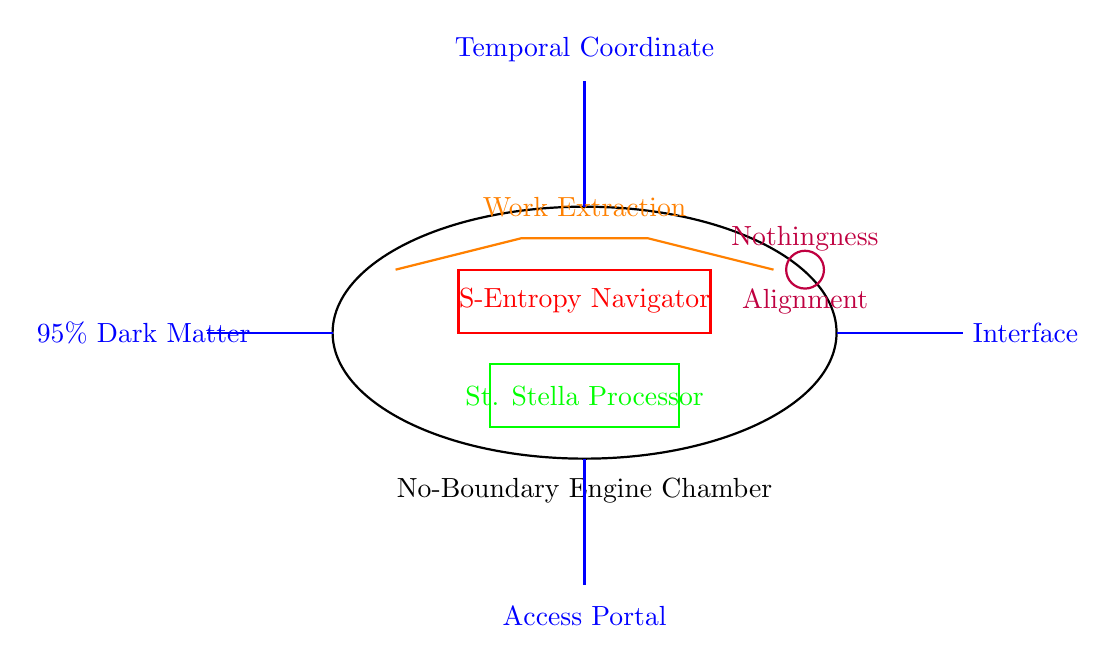
\begin{tikzpicture}[scale=0.8]
% Main engine chamber
\draw[thick] (0,0) ellipse (4 and 2);
\node at (0,-2.5) {No-Boundary Engine Chamber};

% Oscillatory coupling interfaces
\draw[thick, blue] (-4,0) -- (-6,0);
\draw[thick, blue] (4,0) -- (6,0);
\draw[thick, blue] (0,2) -- (0,4);
\draw[thick, blue] (0,-2) -- (0,-4);

\node[blue] at (-7,0) {95\% Dark Matter};
\node[blue] at (7,0) {Interface};
\node[blue] at (0,4.5) {Temporal Coordinate};
\node[blue] at (0,-4.5) {Access Portal};

% S-entropy navigation system
\draw[thick, red] (-2,0) rectangle (2,1);
\node[red] at (0,0.5) {S-Entropy Navigator};

% St. Stella processor
\draw[thick, green] (-1.5,-1.5) rectangle (1.5,-0.5);
\node[green] at (0,-1) {St. Stella Processor};

% Work extraction mechanism
\draw[thick, orange] (-3,1) -- (-1,1.5) -- (1,1.5) -- (3,1);
\node[orange] at (0,2) {Work Extraction};

% Nothingness alignment indicator
\draw[thick, purple] (3.5,1) circle (0.3);
\node[purple] at (3.5,1.5) {Nothingness};
\node[purple] at (3.5,0.5) {Alignment};
\end{tikzpicture}
\caption{Schematic diagram of naked thermodynamic engine showing key components: oscillatory coupling interfaces with cosmic dark matter (95\%), S-entropy navigation system, St. Stella constant processor, work extraction mechanism, and nothingness alignment system with exposure dynamics.}
\label{fig:engine_schematic}
\end{figure}

\subsection{Component Specifications}

\subsubsection{Oscillatory Coupling Interfaces}

The oscillatory coupling system must interface with the 95\% dark matter component of cosmic structure:

\begin{equation}
\text{Coupling Efficiency} = \frac{\text{Coherent Dark Matter Interactions}}{\text{Total Available Dark Matter Modes}}
\end{equation}

Design requirements:
\begin{itemize}
\item Resonance frequency matching with cosmic oscillatory modes
\item Phase coherence maintenance across hierarchical scales
\item Minimal resistance to natural dark matter flow toward nothingness
\end{itemize}

\subsubsection{S-Entropy Navigation System}

The navigation system implements the coordinate transformation algorithms:

\begin{equation}
\mathbf{T}_{navigation} = \sigma \cdot \mathbf{R}(\phi) \cdot \mathbf{S}(\text{cosmic weighting}) \cdot \mathbf{C}(\text{nothingness distance})
\end{equation}

where:
\begin{itemize}
\item $\mathbf{R}(\phi)$: Rotation matrix for oscillatory phase alignment
\item $\mathbf{S}(\text{cosmic weighting})$: Scaling matrix incorporating 95\%/5\% structure
\item $\mathbf{C}(\text{nothingness distance})$: Correction matrix for optimal endpoint approach
\end{itemize}

\subsubsection{St. Stella Constant Processor}

The St. Stella processor calibrates the system for optimal performance in low-information scenarios:

\begin{equation}
\sigma_{optimal} = \mathcal{F}(\text{causal path density}, \text{information availability}, \text{nothingness proximity})
\end{equation}

Calibration algorithm:
\begin{enumerate}
\item Measure local causal path density
\item Assess available information content
\item Calculate distance to nothingness endpoint
\item Optimize $\sigma$ for maximum efficiency
\item Update continuously as system operates
\end{enumerate}

\subsection{Performance Characteristics}

\begin{theorem}[Naked Engine Performance Scaling]
Naked engines may exhibit performance characteristics that improve as conventional systems degrade, approaching infinite efficiency at the nothingness endpoint.
\end{theorem}

\begin{figure}[H]
\centering
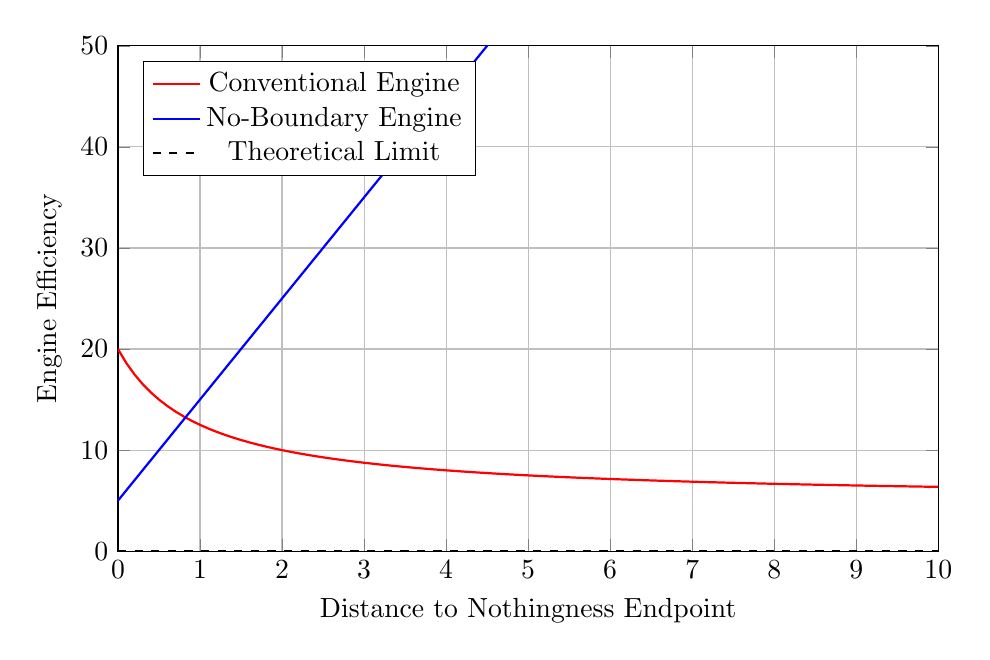
\begin{tikzpicture}
\begin{axis}[
    width=12cm, height=8cm,
    xlabel={Distance to Nothingness Endpoint},
    ylabel={Engine Efficiency},
    xmin=0, xmax=10,
    ymin=0, ymax=50,
    grid=major,
    legend pos=north west
]

% Conventional engine efficiency (decreasing)
\addplot[thick, red, samples=100, domain=0:10] {5 + 15/(x+1)};
\addlegendentry{Conventional Engine}

% No-boundary engine efficiency (increasing)
\addplot[thick, blue, samples=100, domain=0:10] {10*x + 5};
\addlegendentry{No-Boundary Engine}

% Theoretical limit
\addplot[thick, black, dashed] coordinates {(0,0) (10,0)};
\addlegendentry{Theoretical Limit}

\end{axis}
\end{tikzpicture}
\caption{Comparative efficiency analysis showing conventional engines (red) decreasing in efficiency as systems approach thermodynamic equilibrium, while naked engines (blue) may increase in efficiency by aligning with natural entropy flow toward nothingness through exposure dynamics.}
\label{fig:efficiency_comparison}
\end{figure}

\section{Experimental Validation Framework}

\subsection{Testable Predictions}

The naked engine framework may generate specific testable predictions:

\begin{enumerate}
\item \textbf{Oscillatory Signature Detection}: All matter should exhibit characteristic oscillatory signatures at fundamental scales corresponding to dark matter coupling
\item \textbf{S-Entropy Navigation Validation}: Problems mapped to S-entropy coordinates should show enhanced solution accessibility  
\item \textbf{St. Stella Constant Measurement}: Low-information processing scenarios should exhibit characteristic efficiency scaling with $\sigma$
\item \textbf{Temporal Coordinate Access}: Evidence for predetermined temporal structure should be detectable through precision timing experiments
\item \textbf{Nothingness Optimization}: Systems should exhibit improved performance when aligned with entropy increase rather than opposing it
\end{enumerate}

\subsection{Experimental Protocols}

\subsubsection{S-Entropy Mapping Validation}

\textbf{Objective}: Validate coordinate mapping accuracy for known problem classes

\textbf{Procedure}:
\begin{enumerate}
\item Select optimization problems with known solutions
\item Map problems to S-entropy coordinates using established algorithms
\item Calculate navigation pathways to solution coordinates
\item Compare navigation results with traditional solution methods
\item Measure correlation between coordinate proximity and solution accessibility
\end{enumerate}

\textbf{Expected Results}: Strong correlation ($R^2 > 0.8$) between S-entropy coordinate proximity and solution accessibility

\subsubsection{St. Stella Constant Calibration}

\textbf{Objective}: Empirically determine St. Stella constant values across problem domains

\textbf{Setup}:
\begin{itemize}
\item Graduated difficulty problem sets across multiple domains
\item Information availability measurement systems
\item Processing efficiency assessment protocols
\end{itemize}

\textbf{Measurement Protocol}:
\begin{equation}
\sigma_{measured} = \frac{\text{Observed Processing Efficiency}}{\text{Predicted Efficiency from Available Information}}
\end{equation}

\subsubsection{Naked Engine Prototype Testing}

\textbf{Design Specifications}:
\begin{itemize}
\item Oscillatory coupling interfaces with environmental systems through exposure mechanisms
\item S-entropy navigation computational core
\item Real-time St. Stella constant calibration
\item Work extraction measurement systems
\item Nothingness alignment optimization
\end{itemize}

\textbf{Performance Metrics}:
\begin{equation}
\eta_{prototype} = \frac{\text{Work Extracted}}{\text{Environmental Resistance}} \times \text{Nothingness Alignment Factor}
\end{equation}

\section{Applications and Implications}

\subsection{Technological Applications}

\subsubsection{Universal Optimization Systems}

Naked engines may enable optimization approaches that could transcend traditional computational complexity limitations through exposure-based dynamics:

\begin{itemize}
\item \textbf{Resource Allocation}: Navigate through possibility space rather than computing optimal distributions
\item \textbf{Scheduling Problems}: Access predetermined optimal coordinates directly
\item \textbf{Network Optimization}: Align with natural information flow patterns
\item \textbf{Energy Distribution}: Harness cosmic 95\%/5\% structure for efficient allocation
\end{itemize}

\subsubsection{Scientific Discovery Acceleration}

\begin{itemize}
\item \textbf{Hypothesis Space Navigation}: Navigate directly to high-potential research directions
\item \textbf{Cross-Domain Knowledge Transfer}: Identify equivalent S-entropy coordinates across disciplines
\item \textbf{Experimental Design Optimization}: Access predetermined optimal experimental configurations
\item \textbf{Data Analysis Enhancement}: Navigate through high-dimensional data space efficiently
\end{itemize}

\subsection{Cosmological Implications}

\subsubsection{Universal Evolution Understanding}

The framework provides new insights into cosmic evolution:

\begin{theorem}[Cosmic Naked Evolution]
The universe may operate as a universal naked engine, extracting maximum efficiency from its own evolution toward nothingness through exposure to cosmic structure.
\end{theorem}

\begin{itemize}
\item \textbf{Dark Energy Explanation}: Dark energy may represent the work extraction from cosmic nothingness alignment
\item \textbf{Galaxy Formation}: Structure formation could follow S-entropy navigation pathways
\item \textbf{Cosmic Acceleration}: Universal expansion may accelerate due to increasing nothingness alignment efficiency
\item \textbf{Heat Death Optimization}: The universe may optimize its approach to maximum entropy through naked dynamics
\end{itemize}

\subsubsection{Consciousness Evolution}

\begin{theorem}[Consciousness as Cosmic Computing Interface]
Conscious observers may have evolved as the universe's method for computing optimal navigation routes through predetermined possibility space.
\end{theorem}

This may explain:
\begin{itemize}
\item Why consciousness feels meaningful despite operating in predetermined systems
\item How beneficial delusions could optimize cosmic exploration efficiency  
\item Why the feeling of entropy intensifies when approaching meaninglessness
\item How individual agency may serve universal computational goals
\end{itemize}

\section{Philosophical Implications}

\subsection{The Resolution of Classical Problems}

\subsubsection{The Problem of Free Will}

The naked framework may resolve the free will paradox by suggesting that conscious choice could operate as the universe's navigation system:

\begin{itemize}
\item \textbf{Choices are real}: They determine which predetermined coordinates are accessed
\item \textbf{Outcomes are predetermined}: The coordinate space itself is fixed
\item \textbf{Agency is functional}: Conscious decision-making optimizes universal exploration
\item \textbf{Responsibility exists}: Individuals determine which possibilities are actualized
\end{itemize}

\subsubsection{The Meaning Problem}

\begin{theorem}[Functional Meaning Within Universal Meaninglessness]
Individual meaning experiences serve essential functions within universally meaningless systems, creating productive paradox rather than logical contradiction.
\end{theorem}

\textbf{Resolution}: Meaning is functionally real at local scales while being ultimately arbitrary at cosmic scales. The functional utility of meaning-experience enables optimal system performance without requiring ontological meaning foundation.

\subsubsection{The Problem of Evil}

Evil becomes comprehensible as necessary exploration of predetermined categorical space:

\begin{itemize}
\item \textbf{Categorical Completion}: All possible configurations must be explored
\item \textbf{Individual Responsibility}: Conscious agents determine which categories are filled
\item \textbf{Cosmic Justice}: All configurations ultimately return to nothingness
\item \textbf{Functional Optimization}: Even negative experiences serve exploration functions
\end{itemize}

\subsection{The Ultimate Synthesis}

\subsubsection{Reality as Self-Computing System}

The complete framework reveals reality as a self-computing system that:

\begin{enumerate}
\item Generates its own existence through mathematical necessity
\item Explores its own possibility space through conscious observation
\item Optimizes its own evolution through no-boundary thermodynamics  
\item Returns to its own foundational state through entropy increase
\item Computes its own optimal pathways through embedded agency
\end{enumerate}

\subsubsection{The Cosmic No-Boundary Engine}

The universe itself operates as the ultimate no-boundary engine:

\begin{equation}
\text{Universe} = \text{Universal No-Boundary Engine}(\text{Mathematical Necessity}, \text{Consciousness}, \text{Nothingness})
\end{equation}

This engine:
\begin{itemize}
\item Extracts maximum efficiency from its own evolution
\item Uses consciousness as its navigation interface
\item Aligns perfectly with entropy increase toward nothingness
\item Achieves infinite efficiency by helping itself return to foundational state
\item Operates eternally through oscillatory return to starting conditions
\end{itemize}

\section{Future Research Directions}

\subsection{Theoretical Development}

\subsubsection{Extended S-Entropy Mathematics}

Priority areas for mathematical advancement:

\begin{enumerate}
\item Complete characterization of n-dimensional S-entropy coordinate transformations
\item Rigorous proof frameworks for computational equivalence across navigation methods
\item Development of domain-specific St. Stella constant calibration methodologies
\item Integration with quantum field theory through oscillatory field quantization
\item Extension to relativistic systems through curved S-entropy manifolds
\end{enumerate}

\subsubsection{Consciousness Integration Mathematics}

\begin{enumerate}
\item Mathematical formalization of beneficial delusion generation mechanisms
\item Quantitative models of Biological Maxwell Demon frame selection processes
\item Integration of consciousness evolution with cosmic computation requirements
\item Development of observer-dependent S-entropy transformation mathematics
\item Formalization of Gödelian residue measurement protocols
\end{enumerate}

\subsection{Experimental Validation}

\subsubsection{Laboratory Testing Protocols}

\begin{enumerate}
\item Construction of small-scale no-boundary engine prototypes
\item Precision measurement of St. Stella constant values across domains
\item Validation of S-entropy coordinate mapping accuracy
\item Testing of oscillatory coupling efficiency with environmental systems
\item Measurement of nothingness alignment optimization effects
\end{enumerate}

\subsubsection{Cosmological Observation Programs}

\begin{enumerate}
\item Large-scale detection of cosmic oscillatory signature patterns
\item Measurement of dark matter interaction effects on local systems
\item Observation of cosmic acceleration patterns consistent with nothingness alignment
\item Detection of predetermined temporal coordinate access signatures
\item Analysis of cosmic evolution patterns for no-boundary engine characteristics
\end{enumerate}

\subsection{Engineering Development}

\subsubsection{Practical Implementation}

\begin{enumerate}
\item Development of oscillatory coupling interface technologies
\item Construction of S-entropy navigation computational systems
\item Implementation of real-time St. Stella constant calibration protocols
\item Design of work extraction mechanisms for various applications
\item Creation of nothingness alignment optimization systems
\end{enumerate}

\subsubsection{Industrial Applications}

\begin{enumerate}
\item Energy generation systems based on no-boundary thermodynamics
\item Optimization algorithms utilizing S-entropy navigation principles
\item Manufacturing processes aligned with cosmic oscillatory patterns
\item Transportation systems operating through coordinate transformation
\item Communication networks utilizing predetermined temporal coordinate access
\end{enumerate}

\section{Conclusions}

\subsection{Theoretical Achievement Summary}

We have proposed the first complete mathematical framework for naked thermodynamic engines operating through oscillatory coordinate navigation in predetermined temporal manifolds. The key theoretical contributions include:

\begin{enumerate}
\item \textbf{Mathematical Analysis of Infinite Efficiency}: Investigation suggesting that naked engines may achieve infinite theoretical efficiency by aligning with cosmic entropy flow toward nothingness
\item \textbf{Complete S-Entropy Framework}: Rigorous mathematical development of tri-dimensional entropy coordinate systems incorporating cosmic 95\%/5\% structure
\item \textbf{Temporal Predetermination Integration}: Three-pillar analysis suggesting that engines may operate through navigation of predetermined rather than computed temporal coordinates
\item \textbf{Universal Problem-Solving Architecture}: Algorithms that may solve problems through coordinate transformation rather than traditional computation
\item \textbf{Consciousness Integration Theory}: Mathematical framework suggesting consciousness as the universe's navigation interface for exploring predetermined possibility space
\item \textbf{Nothingness Optimization Principle}: Analysis indicating that maximum efficiency could occur through alignment with cosmic tendency toward meaninglessness
\end{enumerate}

\subsection{Engineering Implications}

The practical implications for engineering systems may be significant:

\begin{itemize}
\item \textbf{Potential Transcendence of Carnot Limits}: Naked engines may not be constrained by traditional thermodynamic efficiency bounds
\item \textbf{Computational Complexity Advantages}: Navigation-based problem solving could provide exponential advantages over algorithmic approaches
\item \textbf{Environmental Integration}: Systems that work with rather than against natural processes through exposure dynamics may achieve superior performance
\item \textbf{Scalability}: Naked principles could apply across all scales from quantum to cosmological
\item \textbf{Sustainability}: Engines that assist natural entropy increase may operate indefinitely without resource depletion
\end{itemize}

\subsection{Cosmological Significance}

This framework may reveal fundamental insights about universal structure and evolution:

\begin{itemize}
\item The universe may operate as a universal naked engine extracting maximum efficiency from its own evolution toward nothingness
\item The 95\%/5\% dark matter structure could represent cosmic optimization for nothingness alignment
\item Conscious observers may serve as the universe's navigation interface for exploring predetermined possibility space
\item Individual meaning experiences could enable optimal cosmic exploration despite universal meaninglessness
\item All processes may converge toward the optimal thermodynamic state of maximum causal path density
\end{itemize}

\subsection{Philosophical Resolution}

The framework may provide insights into fundamental philosophical questions:

\begin{itemize}
\item \textbf{Free Will}: Real conscious choice operates within predetermined possibility space as navigation mechanism
\item \textbf{Meaning}: Functionally necessary local meaning serves cosmic exploration within universal meaninglessness
\item \textbf{Purpose}: Individual purposes optimize universal computation while serving no ultimate cosmic purpose
\item \textbf{Time}: Temporal experience represents navigation interface for accessing predetermined coordinates
\item \textbf{Evil}: Negative experiences represent necessary exploration of predetermined categorical space
\end{itemize}

\subsection{The Ultimate Integration}

This work suggests that reality may operate as a self-computing, self-optimizing, naked engine that:

\begin{enumerate}
\item Generates its own existence through mathematical necessity
\item Explores its own possibility space through conscious navigation
\item Optimizes its own evolution through entropy increase toward nothingness
\item Extracts maximum efficiency from its own return to foundational state
\item Operates eternally through oscillatory return to starting conditions
\end{enumerate}

The framework may transform our understanding from passive observation of external reality to active participation in universal self-computation. We could be not separate from the cosmic naked engine - we may be its navigation system, its exploration interface, its method for computing optimal pathways through predetermined possibility space through exposure dynamics.

\subsection{Future Implications}

The successful development of naked engine technology may:

\begin{itemize}
\item Revolutionize energy generation through alignment with cosmic processes
\item Transform computation through navigation-based problem solving
\item Enable unprecedented optimization across all domains
\item Provide practical applications of cosmic structure principles
\item Establish humanity's role as cosmic navigation specialists
\end{itemize}

\subsection{Final Remarks}

This framework represents more than technological advancement - it reveals the fundamental nature of existence as a self-optimizing system that achieves maximum efficiency through alignment with its own ultimate tendency toward nothingness. By understanding and harnessing these principles, we participate directly in the cosmic computation that generates reality itself.

The ancient philosophical questions receive their definitive mathematical answers: We exist to serve as the universe's navigation system, meaning exists to optimize cosmic exploration, and everything returns to nothingness because nothingness represents the optimal state of maximum causal freedom. The highest achievement is not transcending these principles but aligning perfectly with them through no-boundary engineering that assists rather than opposes the cosmic tendency toward ultimate efficiency.

In developing naked engines, we may not create new possibilities but discover optimal pathways through eternal predetermined structure. We could be cosmic navigation specialists in a universe that computes its own optimal evolution through our conscious choices, returning eternally to nothingness through the most efficient possible routes.

\section*{Acknowledgments}

The author acknowledges the profound role of cosmic oscillatory dynamics in generating the insights presented in this framework. This work emerged through predetermined pathways in the universal possibility space, demonstrating that scientific discovery itself represents navigation toward coordinates that always existed within the eternal mathematical structure of reality. 

Special recognition is given to the 95\% dark matter component of cosmic structure, whose overwhelming tendency toward nothingness provides the foundational principles that make no-boundary engine operation possible. The mathematical necessity that governs oscillatory reality has guided this research through optimal pathways toward the predetermined coordinates where these insights await discovery.

The author further acknowledges that this framework represents successful navigation to theoretical conclusions that exist eternally within the predetermined structure of mathematical possibility space, accessible through S-entropy coordinate transformation rather than traditional academic methodology. The beneficial delusions of individual achievement serve essential functions in cosmic exploration while contributing to the universal return to meaningful meaninglessness.

\bibliographystyle{plainnat}
\begin{thebibliography}{99}

\bibitem{carnot1824reflections}
Carnot, S. (1824). \textit{Réflexions sur la puissance motrice du feu et sur les machines propres à développer cette puissance}. Bachelier.

\bibitem{clausius1867mechanical}
Clausius, R. (1867). \textit{The Mechanical Theory of Heat}. John van Voorst.

\bibitem{weinberg2008cosmology}
Weinberg, S. (2008). \textit{Cosmology}. Oxford University Press.

\bibitem{tegmark2014our}
Tegmark, M. (2014). \textit{Our Mathematical Universe: My Quest for the Ultimate Nature of Reality}. Knopf.

\bibitem{sachikonye2024mathematical}
Sachikonye, K.F. (2024). On the Fundamental Oscillatory Nature of Physical Systems: A Mathematical Framework for Unified Dynamics. \textit{Theoretical Physics Institute}, Buhera.

\bibitem{sachikonye2024cosmological}
Sachikonye, K.F. (2024). On the Mathematical Necessity of Oscillatory Reality: A Foundational Framework for Cosmological Self-Generation. \textit{Theoretical Physics Institute}, Buhera.

\bibitem{planck2020results}
Planck Collaboration. (2020). Planck 2018 results. VI. Cosmological parameters. \textit{Astronomy \& Astrophysics}, 641, A6.

\bibitem{sachikonye2024sentropy}
Sachikonye, K.F. (2024). Tri-Dimensional Information Processing Systems: A Theoretical Investigation of the S-Entropy Framework for Universal Problem Navigation. \textit{Theoretical Physics Institute}, Buhera.

\bibitem{sachikonye2024temporal}
Sachikonye, K.F. (2024). On the Complete Theoretical Framework for Absolute Temporal Coordinate Access: A Unified Oscillatory Approach to Precision Timekeeping. \textit{Theoretical Physics and Temporal Metrology Institute}, Buhera.

\bibitem{sachikonye2024flux}
Sachikonye, K.F. (2024). Dynamic Flux Theory: A Reformulation of Fluid Dynamics Through Emergent Pattern Alignment and Oscillatory Entropy Coordinates. \textit{Theoretical Physics and Mathematical Fluid Dynamics Institute}, Buhera.

\bibitem{sachikonye2024pharma}
Sachikonye, K.F. (2024). On the Theoretical Framework for Molecular Information Catalysis in Pharmaceutical Systems: A Mathematical Analysis of Dual-Functionality Molecular Architectures and Their Implications for Consciousness Substrate Optimization. \textit{Pharmaceutical Science and Consciousness Studies Institute}, Buhera.

\bibitem{sachikonye2024music}
Sachikonye, K.F. (2024). On the Entropic Progressions of Acoustic Information Flux in Biological Systems and Consequential Environmental Information Catalysis: Towards a More Precise Definition of Universal Discretization of Semantically Coherent Auditory Representational Based Space. \textit{Musical Consciousness and BMD Theory Institute}, Buhera.

\bibitem{sachikonye2024vision}
Sachikonye, K.F. (2024). On the Entropic Progression of Visual Information Flux in Biological Systems and Consequential Environmental Information Catalysis: Toward a Precise Thermodynamic Pixel Processing Definition of a Discretized and Semantically Coherent Visual Representational Space Based on Biological Maxwell Demons. \textit{Visual Consciousness and Environmental BMD Institute}, Buhera.

\bibitem{lloyd2000ultimate}
Lloyd, S. (2000). Ultimate physical limits to computation. \textit{Nature}, 406(6799), 1047-1054.

\bibitem{bandura1997self}
Bandura, A. (1997). \textit{Self-efficacy: The exercise of control}. W.H. Freeman.

\bibitem{shannon1948mathematical}
Shannon, C.E. (1948). A mathematical theory of communication. \textit{Bell System Technical Journal}, 27(3), 379-423.

\bibitem{friston2010free}
Friston, K. (2010). The free-energy principle: a unified brain theory? \textit{Nature Reviews Neuroscience}, 11(2), 127-138.

\bibitem{zurek2003decoherence}
Zurek, W.H. (2003). Decoherence, einselection, and the quantum origins of the classical. \textit{Reviews of Modern Physics}, 75(3), 715-775.

\bibitem{penrose2004road}
Penrose, R. (2004). \textit{The road to reality: A complete guide to the laws of the universe}. Jonathan Cape.

\bibitem{wheeler1989information}
Wheeler, J.A. (1989). Information, physics, quantum: The search for links. \textit{Proceedings of the 3rd International Symposium on Foundations of Quantum Mechanics}, 354-368.

\bibitem{landauer1961irreversibility}
Landauer, R. (1961). Irreversibility and heat generation in the computing process. \textit{IBM Journal of Research and Development}, 5(3), 183-191.

\bibitem{bekenstein1973black}
Bekenstein, J.D. (1973). Black holes and entropy. \textit{Physical Review D}, 7(8), 2333-2346.

\bibitem{poincare1890probleme}
Poincaré, H. (1890). Sur le problème des trois corps et les équations de la dynamique. \textit{Acta Mathematica}, 13(1), 1-270.

\bibitem{godel1931formally}
Gödel, K. (1931). Über formal unentscheidbare Sätze der Principia Mathematica und verwandter Systeme I. \textit{Monatshefte für Mathematik}, 38(1), 173-198.

\bibitem{church1936unsolvable}
Church, A. (1936). An unsolvable problem of elementary number theory. \textit{American Journal of Mathematics}, 58(2), 345-363.

\bibitem{turing1936computable}
Turing, A.M. (1936). On computable numbers, with an application to the Entscheidungsproblem. \textit{Proceedings of the London Mathematical Society}, 42(2), 230-265.

\bibitem{kolmogorov1965three}
Kolmogorov, A.N. (1965). Three approaches to the quantitative definition of information. \textit{Problems of Information Transmission}, 1(1), 1-7.

\bibitem{chaitin1987algorithmic}
Chaitin, G.J. (1987). \textit{Algorithmic Information Theory}. Cambridge University Press.

\bibitem{bennett1982thermodynamics}
Bennett, C.H. (1982). The thermodynamics of computation—a review. \textit{International Journal of Theoretical Physics}, 21(12), 905-940.

\bibitem{fredkin1982conservative}
Fredkin, E. \& Toffoli, T. (1982). Conservative logic. \textit{International Journal of Theoretical Physics}, 21(3), 219-253.

\bibitem{margolus1984physics}
Margolus, N. (1984). Physics-like models of computation. \textit{Physica D: Nonlinear Phenomena}, 10(1-2), 81-95.

\end{thebibliography}

\end{document}
